% This is "sig-alternate.tex" V2.1 April 2013

\documentclass{sig-alternate-05-2015}
\usepackage{array}
\newcolumntype{L}[1]{>{\raggedright\let\newline\\\arraybackslash\hspace{0pt}}m{#1}}
\newcolumntype{C}[1]{>{\centering\let\newline\\\arraybackslash\hspace{0pt}}m{#1}}
\newcolumntype{R}[1]{>{\raggedleft\let\newline\\\arraybackslash\hspace{0pt}}m{#1}}

\begin{document}

\title{Interactive Model Serving for Regulatory Genomics}


\numberofauthors{4}

\author{
\alignauthor
Alyssa Morrow \\
       \email{akmorrow@berkeley.edu}
\alignauthor
Devin Petersohn \\
       \email{devin.petersohn@berkeley.edu}
\alignauthor Anthony Joseph \\
       \email{adj@berkeley.edu}
\and  % use '\and' if you need 'another row' of author names
\alignauthor Nir Yosef \\
       \email{nir.yosef@berkeley.edu}
}

\maketitle
\begin{abstract}
Current pipelines for training machine learning models on genomic and epigenetic datasets lack resources to scale to current datasets sizes. Furthermore, pipelines for testing and evaluating these machine learning models are segmented, as they require users to separately test pipelines and evaluate their methods using disjunct software. In this paper we survey current workflows for training, testing and evaluating genomic machine learning models and provide an alternative solution to connecting the dots between these processes. More specifically, we present a complete fast and interactive pipeline that allows users to save prebuilt models and evaluate these models in a visual environment with low latency.
\end{abstract}


\printccsdesc

\keywords{Genomics; Model Serving; Transcription Factors}

\section{Introduction}
Regulatory genomics is a field of research that works to connect the function of DNA sequence, DNA interacting proteins and cell environment with gene expression. Understanding and predicting regulatory function is important, as it allows clinicians to predict the effect of an individual's genetic variants on their health and well being. Currently, there exist many different computational methods for prediction of regulatory function, including convolutional neural networks and kernels with SVM classification \cite{alipanahi2015predicting}, \cite{kelley2016basset}.  Datasets used to predict regulatory function are massive, reaching 15 TB in the ENCODE consortium \cite{encode2004encode}. However, these datasets are noisy, and thus analysis of regulatory predictions often require a human in the loop to visually interpret predictions against ground truth datasets produced in datasets such as ENCODE. \\

Current pipelines for training and analyzing regulatory genomic models include a segmented group of steps that are exclusive and require preprocessing between each stage. For example, the state-of-the-art pipeline involves executing a locally run algorithm, such as a kernel method or neural network, built for a single machine. Users who are interested in predicting on a particular sequence face multiple challenges. Because the state-of-the-art methods are not built to scale past a single machine, users must first subselect a number of regions of the genome to train on specific to their hardware capabilities. After subselecting and training on that data, the user would then load these regions into a single node visualization tool, such as \cite{igv2011}, and repeat the preprocessing step to validate their model. A demonstration of the workflow pipeline required using currently available tools can be shown in Figure~\ref{fig:strawmanPipeline}.

\begin{figure}[b]
  \label{fig:strawmanPipeline}
  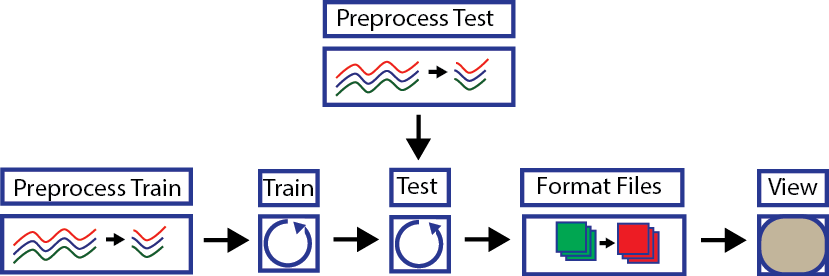
\includegraphics[width=0.5\textwidth]{figures/strawman.png}
  \caption{Stawman pipeline for training and evaluating model.}
\end{figure}

Currently, there is no infrastructure available for users to upload and predict on their sequences in real time. In practice, this infrastructure is not available, due in part to the difficulty of serving models at a large scale. Genomic data typically ranges on the order of 100's of MB to 10's of GB of data. The models are typically built with 10's of GB to 100's of GB of data, creating a unique challenge when trying to achieve interactive model serving speeds.

In the paper, we describe an end-to-end pipeline that efficiently computes and predicts on user provided sequences while maintaining seamless integration between processing steps. In our previous work, we use a scalable and parallel algorithm to efficiently compute protein binding sites without the use of specialized hardware \cite{tfbinding}. Here, we utilize this algorithm to predict from regulatory datasets, and provide a full analysis pipeline to visualize results. This novel pipeline allows users to interactively predict on regions of interest in a query genome. We compare our pipeline to the current state-of-the-art approaches on a single node, and then analyze pipeline latency at scale. \\


\begin{figure}
  \label{fig:strawmanPipeline}
  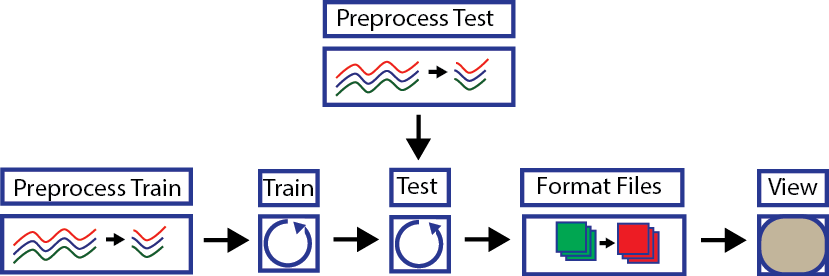
\includegraphics[width=0.5\textwidth]{figures/strawman.png}
  \caption{Stawman pipeline for training and evaluating model.}
\end{figure}

\section{Background}
Existing infrastructure for model prediction and serving is not built for scalable computing environments. In this section, we describe the current state-of-the-art pipeline components.

\subsection{Algorithms}
Current algorithms for predicting on regulatory genomic datasets include neural networks and string kernels with SVM classification.

These methods train on small portions of the genome. For example, a neural net implementation DeepBind subselects 10,000 sequences to predict protein binding sites. Similarly, Kernel SVM uses 10,000 sequence to learn a classifier. Both tools are intended to run on a single machine. \\

\subsection{Evaluation Tools}
Main interative tools for evaluating algorithms discussed above include visualization tools, such as University of Santa Cruz Genome Browser and IGV \cite{ucscbrowser}, \cite{igv2011}. IGV is a desktop application that allows visualization of a wide variety of genomic datasets. IGV is used by clinicians and researchers to verify anomalies in their data and verify predictions on original raw genomic datasets. IGV does not support integrated visualization of predictive models, so users attempting to perform visual analysis of models using heterogeneous datasets must predict outside of the visualization tool.

\section{Architecture}
In this section, we outline our design for an end-to-end machine learning pipeline on epigenetic datasets. Our implementation builds upon previously built distributed genomics tools such as ADAM, Mango and Endive, which are described below. Finally, we will demonstrate how these tools can be connected together to create an end-to-end pipeline for machine learning tasks. \\

\subsection{ADAM: Distributed Genomic Workloads}
ADAM is a framework for processing genomic data, and is built to run in the Spark ecosystem \cite{adam}. ADAM uses distributed abstractions in Spark to batch process raw genomic datasets in parallel. More importantly, ADAM provides standardized schemas intended for various types of genomic datasets, presented in a narrow waist design that can be easily accessible by external applications. A figure of schema design is shown in Figure X. Important schemas that are used for epigenetic datasets include Alignment Record, Features, and Variant schemas. These schemas are demonstrated in Figure~\ref{fig:adam}. \\

 \begin{figure}
   \label{fig:adam}
   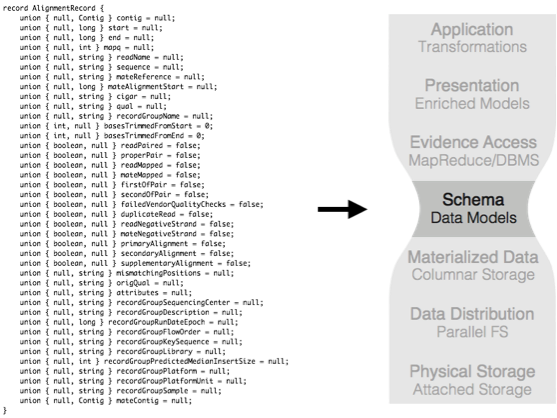
\includegraphics[width=0.5\textwidth]{figures/adamSchema.png}
   \caption{Example of AlignmentRecord schema used in
   Narrow waist design. Schema layer can be swapped in or
   Out for genomic workloads and substituted in for legacy file formats.}
 \end{figure}

In the use case of training a machine learning model on genomic data, ADAM is used to format training
 datasets into standardized schemas that can be saved and read by the hadoop ecosystem. These formats can then be read by ADAM and joined or aggregated to preprocess datasets into records read by a machine learning model.


\subsection{Mango: Genome Visualization}

\begin{figure}
  \label{fig:mango}
  
\includegraphics[width=0.5\textwidth]{figures/mango.png}
  \caption{Stack diagram for Mango architecture. Mango is built on ADAM and Spark, allowing users to perform and visualize fine grained queries on large genomic files.
  Endive}
\end{figure}

Mango is a distributed genome visualization browser that selectively materializes and organizes genomic data to provide fast and fine grained queries on datasets. Mango materializes data from persistent storage as the user requests different regions of the genome. This data is efficiently partitioned and organized in memory using a specialized RDD structure built upon interval trees. This interval based organizational structure supports ad hoc queries, enabling exploratory interaction with genomic data.  Mango is built on top of Spark and ADAM. A demonstration of Mango architecture can be seen in Figure~\ref{fig:mango}. Mango is implemented in three layers, namely, the cluster, server and client. In the cluster layer, Mango is built on ADAM and Spark, allowing users to perform and visualize fine grained queries on large genomic files. The server layer reduces and samples queries so that users can visualize their queries in an efficient and interpretable manner.


\subsection{Endive: Regulatory Machine Learning Abstractions}
Our machine learning tool, called Endive, provides core abstract stages for building end-to-end machine learning pipelines to train and evaluate on genomic datasets. These stages include data preprocessing, featurization, and various solvers apt for genomic workloads. These stages in a machine learning pipeline can be mixed and matched to create novel pipelines tailored to a genomic prediction task of interest.
Preprocessing in Endive involves taking raw genomic data and parsing it into a vector of numeric values which can be directly read by a machine learning model. These preprocessing steps include formatting datasets as well as joining together heterogeneous datasets into one record based on coordinate location in the genome.
Featurization steps in Endive involve taking preprocessed datasets created in the preprocessing stage and transforming these records to explicit features that can be trained and tested on. Table~\ref{table:featurization} contains examples of these featurization steps. These computed features can then be fed into a choice of solvers developed in Keystone ML to train these machine learning models \cite{keystone}.

\begin{table}[t]
\centering
\caption{Featurization Techniques}
\label{table:featurization}
\begin{tabular}{| L{2cm} | L{1.45cm} | L{2cm} | L{1.75cm} |}
\hline
Featurization Technique & Datasets & Description & Usage
\\ \hline
Read Wavelets \newline
\cite{wavelets}         & DNA-seq, RNA-seq           & Iteratively quantifies read pileup                                 & Identification of genomic footprints \\ \hline
Kernel Approximation
\cite{tfbinding} & Sequence, DNA-seq,
RNA-seq & Approximates kernel matrix through random features & Generic, Widely applicable \cite{alipanahi2015predicting}                                       \\ \hline
K-mer counts & Sequence & Counts the number of times each motif
appears in a sequence of length k & Identification
of motifs, quantification of sequence similarity \\ \hline
\end{tabular}
\end{table}

\begin{figure}
  \label{fig:pipeline}
  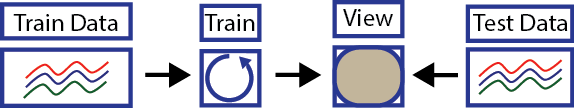
\includegraphics[width=0.5\textwidth]{figures/ourpipeline.png}
  \caption{Pipeline overview. We eliminate preprocessing and file formatting steps.}
\end{figure}


\section{Experiments}
For preliminary results, we train a model predicting protein binding sites using the kernel approximation featurization method described in Table~\ref{table:featurization}  from ENCODE datasets using DNA sequence. This model was solved using Keystone ML's Weighted Least Squares estimator, which accounts for large class imbalance of positive binding sites across the genome. This model was trained both locally on a small dataset as well as in a distributed environment on a large (200 million) dataset. These models generated a 4 MB model to be tested on new datasets. This model was loaded into the Mango genome browser and was used to interactively predict on DNA reference sequences as the user scrolled to new regions of the browser.


\subsection{Local Comparison}
For a straw man comparison, we took the state of the art pipeline used to train and analyze protein binding sites on a local computer. We trained a model on 15,000 DNA sequences to predict the location of binding sites of the EGR1 transcription factor, then visualizing the results in a genome browser, IGV. Because the models were too expensive to train locally, we train both straw man and our models on one machine with 24 Xeon processors, and 256 GB of RAM and 1 Nvidia Tesla K20c GPU. The state of the art in transcription factor binding is DeepBind, and uses a neural net. Previously, we demonstrated the improved accuracy and training time of the Convolutional Kitchen Sink over DeepBind's neural net implementation \cite{tfbinding}. The results of the runtime experiment for serving the model are displayed in Figure~\ref{fig:igvcomp}. A significant difference between Model Serving with Mango and using IGV is that with Mango, we are able to use Servable Chunks, which are defined in the user space. With IGV, there is no way to perform this prediction without completing the entire prediction over the whole search space.

\begin{figure}
  \label{fig:igvcomp}
  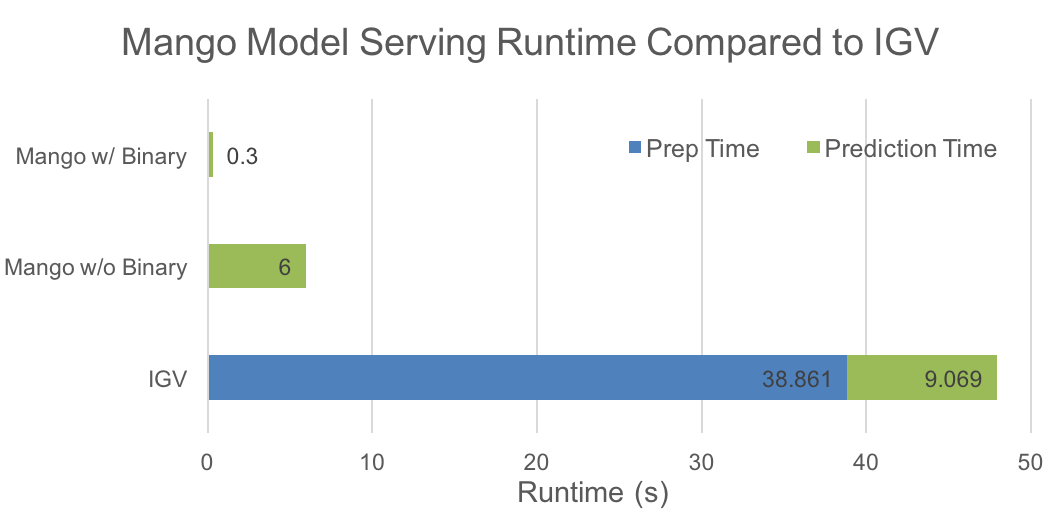
\includegraphics[width=0.5\textwidth]{figures/mangoVsIGV.png}
  \caption{Runtime comparison with IGV and DeepBind}
\end{figure}

In the bwowser, we test on region sizes of 2000 bp, 2000 bp, 4000bp, 8000bp and 16000bp. Initially, our results were on the order of 6 seconds, which is sub-optimal for an application with a user interface. The results in Figure~\ref{fig:igvcomp} show a difference between our implementation with and without the binary pre-fetching approach. Binary pre-fetching allows us to rule out a significant part of the Servable Chunk.



\subsection{Whole Genome Model Serving}
For our second experiment, we trained on the full genome, consisting of 200 million sequences consisting of 640 GB to predict binding sites for protein EGR1. We visualize all raw data related to the model prediction problem, specifically DNA sequence and Dnase hypersensitivity files. Training the model took 58 minutes parallized across 16 nodes with Intel E5-2670 2.6 GHz 8 core CPU, 256 GB RAM and 4 1-TB HDFS hard drives. The generated model was saved and loaded into Mango to visualize predictions on raw datasets. Minimum, maximum and mean times to predict on new sequences using the sparcity model explained above is show in Table~\ref{table:fullGenome}. As in the local experiments, we test on region sizes of 2000 bp, 2000 bp, 4000bp, 8000bp and 16000bp. \\

The mean exectution time of 402.31 ms meets interactive requirements of 500ms. However, maximum execution time of 3.98s is too high for interactive time.

\begin{table}
\centering
% \vspace{-0.4cm}
\caption{Minimum, maximum and mean prediction response times for transcription factor EGR1.}
\label{table:fullGenome}
% \hspace*{-0.96cm}
\begin{tabular}{|l|l|l|}
\hline
\textbf{Min} & \textbf{Max} & \textbf{Mean} \\ \hline
3.09 ms & 3.98 s & 402.31 ms  \\ \hline
\end{tabular}
\end{table}

Table~\ref{table:fullGenome} shows the results of this experiment. Even on a significantly larger model, we averaged prediction times in the 400ms range. This is close to the level required for interactive applications, particularly applications with a user interface.

\section{Conclusion}
There is a need in the scientific community for a tool that accepts user data uploaded from a browser. Genomic data presents new challenges to model serving. Currently, there is no infrastructure in place to allow users to upload and interactively predict on their data. Because of the scale, interactivity is a difficult challenge. In this paper, we describe a novel approach to model serving for extremely large datasets. The process involves using Servable Chunks defined in user space to cut down on network and model prediction overheads. Additionally, we describe a binary pre-fetching approach to achieve close-to-interactive prediction times. Further optimization can be achieved in many parts of the pipeline. We are first interested in taking further advantage of sparsity of the positive predictions. We can do this in a couple of obvious ways. First, we can build a Hidden Markov Model (HMM) on the sequences and uploaded data, allowing us further optimization on the basis of where they will likely look for results next. With this information, we can further pre-fetch results to get them ready for the user's change in prediction window. Second, we can take a sampling method that does not examine the entire sequence. For this sampling method, we do not need to sample from a positive prediction to know that there is a positive prediction nearby. By using a sampling method, we can cut down on the size of the data being predicted and significantly reduce the prediction time. A combination of these two techniques with the Binary Pre-fetching is likely to improve the runtime of predictions to interactive levels.

There are several other future components we would like to add to this model serving pipeline. Another important aspect we would like to incorporate into our approach is a dynamic update component. When users upload their sequences, we want to improve our model with their data. Additionally, we would like to share the computation with users. If we can share some of the computation with users, we can significantly reduce the amount of network traffic and computation load on our server. There are several challenges with this model. First, users will have access to the prediction model, which can be problematic for security. In the case that we use private data for predicting these sequences, we do not want users to be able learn the original training data composition based on our model. Before we can split computation, we need a way to obscure the training data so that our private training data is not compromised.

In order to make this a usable application, we will need to develop the model serving application into a full pipeline. Specifically, we will need to include preprocessing for the data being uploaded so that it is always in the correct format. The field of genomics suffers from an incredibly wide range of formats and file types. This presents challenges when building tools; each format has nuances that require unique methods to handle them. Additionally, users should be able to download the full prediction over their entire sequence once it's complete.

\bibliographystyle{abbrv}
\bibliography{paperRef}

\end{document}
